%!TeX root=../sensetop.tex
\chapter[Chapter \thechapter]{}
\lettrine[lines=4,lraise=0.3]{M}{rs} Dashwood did not hear unmoved the vindication of her former favourite. She rejoiced in his being cleared from some part of his imputed guilt;—she was sorry for him;—she wished him happy. But the feelings of the past could not be recalled.—Nothing could restore him with a faith unbroken—a character unblemished, to Marianne. Nothing could do away the knowledge of what the latter had suffered through his means, nor remove the guilt of his conduct towards Eliza. Nothing could replace him, therefore, in her former esteem, nor injure the interests of Colonel Brandon.

Had Mrs Dashwood, like her daughter, heard Willoughby’s story from himself—had she witnessed his distress, and been under the influence of his countenance and his manner, it is probable that her compassion would have been greater. But it was neither in Elinor’s power, nor in her wish, to rouse such feelings in another, by her retailed explanation, as had at first been called forth in herself. Reflection had given calmness to her judgment, and sobered her own opinion of Willoughby’s deserts;—she wished, therefore, to declare only the simple truth, and lay open such facts as were really due to his character, without any embellishment of tenderness to lead the fancy astray.

In the evening, when they were all three together, Marianne began voluntarily to speak of him again;—but that it was not without an effort, the restless, unquiet thoughtfulness in which she had been for some time previously sitting—her rising colour, as she spoke,—and her unsteady voice, plainly showed.

»I wish to assure you both,« said she, »that I see every thing—as you can desire me to do.«

Mrs Dashwood would have interrupted her instantly with soothing tenderness, had not Elinor, who really wished to hear her sister’s unbiased opinion, by an eager sign, engaged her silence. Marianne slowly continued,—

»It is a great relief to me—what Elinor told me this morning—I have now heard exactly what I wished to hear.«—For some moments her voice was lost; but recovering herself, she added, and with greater calmness than before—»I am now perfectly satisfied, I wish for no change. I never could have been happy with him, after knowing, as sooner or later I must have known, all this.—I should have had no confidence, no esteem. Nothing could have done it away to my feelings.«

»I know it—I know it,« cried her mother. »Happy with a man of libertine practices!—With one who so injured the peace of the dearest of our friends, and the best of men!—No—my Marianne has not a heart to be made happy with such a man!—Her conscience, her sensitive conscience, would have felt all that the conscience of her husband ought to have felt.«

Marianne sighed, and repeated, »I wish for no change.«

»You consider the matter,« said Elinor, »exactly as a good mind and a sound understanding must consider it; and I dare say you perceive, as well as myself, not only in this, but in many other circumstances, reason enough to be convinced that your marriage must have involved you in many certain troubles and disappointments, in which you would have been poorly supported by an affection, on his side, much less certain. Had you married, you must have been always poor. His expensiveness is acknowledged even by himself, and his whole conduct declares that self-denial is a word hardly understood by him. His demands and your inexperience together, on a small, very small income, must have brought on distresses which would not be the \textit{less} grievous to you, from having been entirely unknown and unthought of before. \textit{Your} sense of honour and honesty would have led you, I know, when aware of your situation, to attempt all the economy that would appear to you possible: and, perhaps, as long as your frugality retrenched only on your own comfort, you might have been suffered to practice it, but beyond that—and how little could the utmost of your single management do to stop the ruin which had begun before your marriage? Beyond \textit{that}, had you endeavoured, however reasonably, to abridge \textit{his} enjoyments, is it not to be feared, that instead of prevailing on feelings so selfish to consent to it, you would have lessened your own influence on his heart, and made him regret the connection which had involved him in such difficulties?«

Marianne’s lips quivered, and she repeated the word »Selfish?« in a tone that implied—»do you really think him selfish?«

»The whole of his behaviour,« replied Elinor, »from the beginning to the end of the affair, has been grounded on selfishness. It was selfishness which first made him sport with your affections; which afterwards, when his own were engaged, made him delay the confession of it, and which finally carried him from Barton. His own enjoyment, or his own ease, was, in every particular, his ruling principle.«

»It is very true. \textit{My} happiness never was his object.«

»At present,« continued Elinor, »he regrets what he has done. And why does he regret it?—Because he finds it has not answered towards himself. It has not made him happy. His circumstances are now unembarrassed—he suffers from no evil of that kind; and he thinks only that he has married a woman of a less amiable temper than yourself. But does it follow that had he married you, he would have been happy?—The inconveniences would have been different. He would then have suffered under the pecuniary distresses which, because they are removed, he now reckons as nothing. He would have had a wife of whose temper he could make no complaint, but he would have been always necessitous—always poor; and probably would soon have learned to rank the innumerable comforts of a clear estate and good income as of far more importance, even to domestic happiness, than the mere temper of a wife.«

»I have not a doubt of it,« said Marianne; »and I have nothing to regret—nothing but my own folly.«

»Rather say your mother’s imprudence, my child,« said Mrs Dashwood; »\textit{she} must be answerable.«

Marianne would not let her proceed;—and Elinor, satisfied that each felt their own error, wished to avoid any survey of the past that might weaken her sister’s spirits; she, therefore, pursuing the first subject, immediately continued,

»\textit{One} observation may, I think, be fairly drawn from the whole of the story—that all Willoughby’s difficulties have arisen from the first offence against virtue, in his behaviour to Eliza Williams. That crime has been the origin of every lesser one, and of all his present discontents.«

Marianne assented most feelingly to the remark; and her mother was led by it to an enumeration of Colonel Brandon’s injuries and merits, warm as friendship and design could unitedly dictate. Her daughter did not look, however, as if much of it were heard by her.

Elinor, according to her expectation, saw on the two or three following days, that Marianne did not continue to gain strength as she had done; but while her resolution was unsubdued, and she still tried to appear cheerful and easy, her sister could safely trust to the effect of time upon her health.

Margaret returned, and the family were again all restored to each other, again quietly settled at the cottage; and if not pursuing their usual studies with quite so much vigour as when they first came to Barton, at least planning a vigorous prosecution of them in future.

Elinor grew impatient for some tidings of Edward. She had heard nothing of him since her leaving London, nothing new of his plans, nothing certain even of his present abode. Some letters had passed between her and her brother, in consequence of Marianne’s illness; and in the first of John’s, there had been this sentence:—»We know nothing of our unfortunate Edward, and can make no enquiries on so prohibited a subject, but conclude him to be still at Oxford;« which was all the intelligence of Edward afforded her by the correspondence, for his name was not even mentioned in any of the succeeding letters. She was not doomed, however, to be long in ignorance of his measures.

Their man-servant had been sent one morning to Exeter on business; and when, as he waited at table, he had satisfied the inquiries of his mistress as to the event of his errand, this was his voluntary communication,—

»I suppose you know, ma’am, that Mr Ferrars is married.«

\begin{figure}[tbph]
\centering
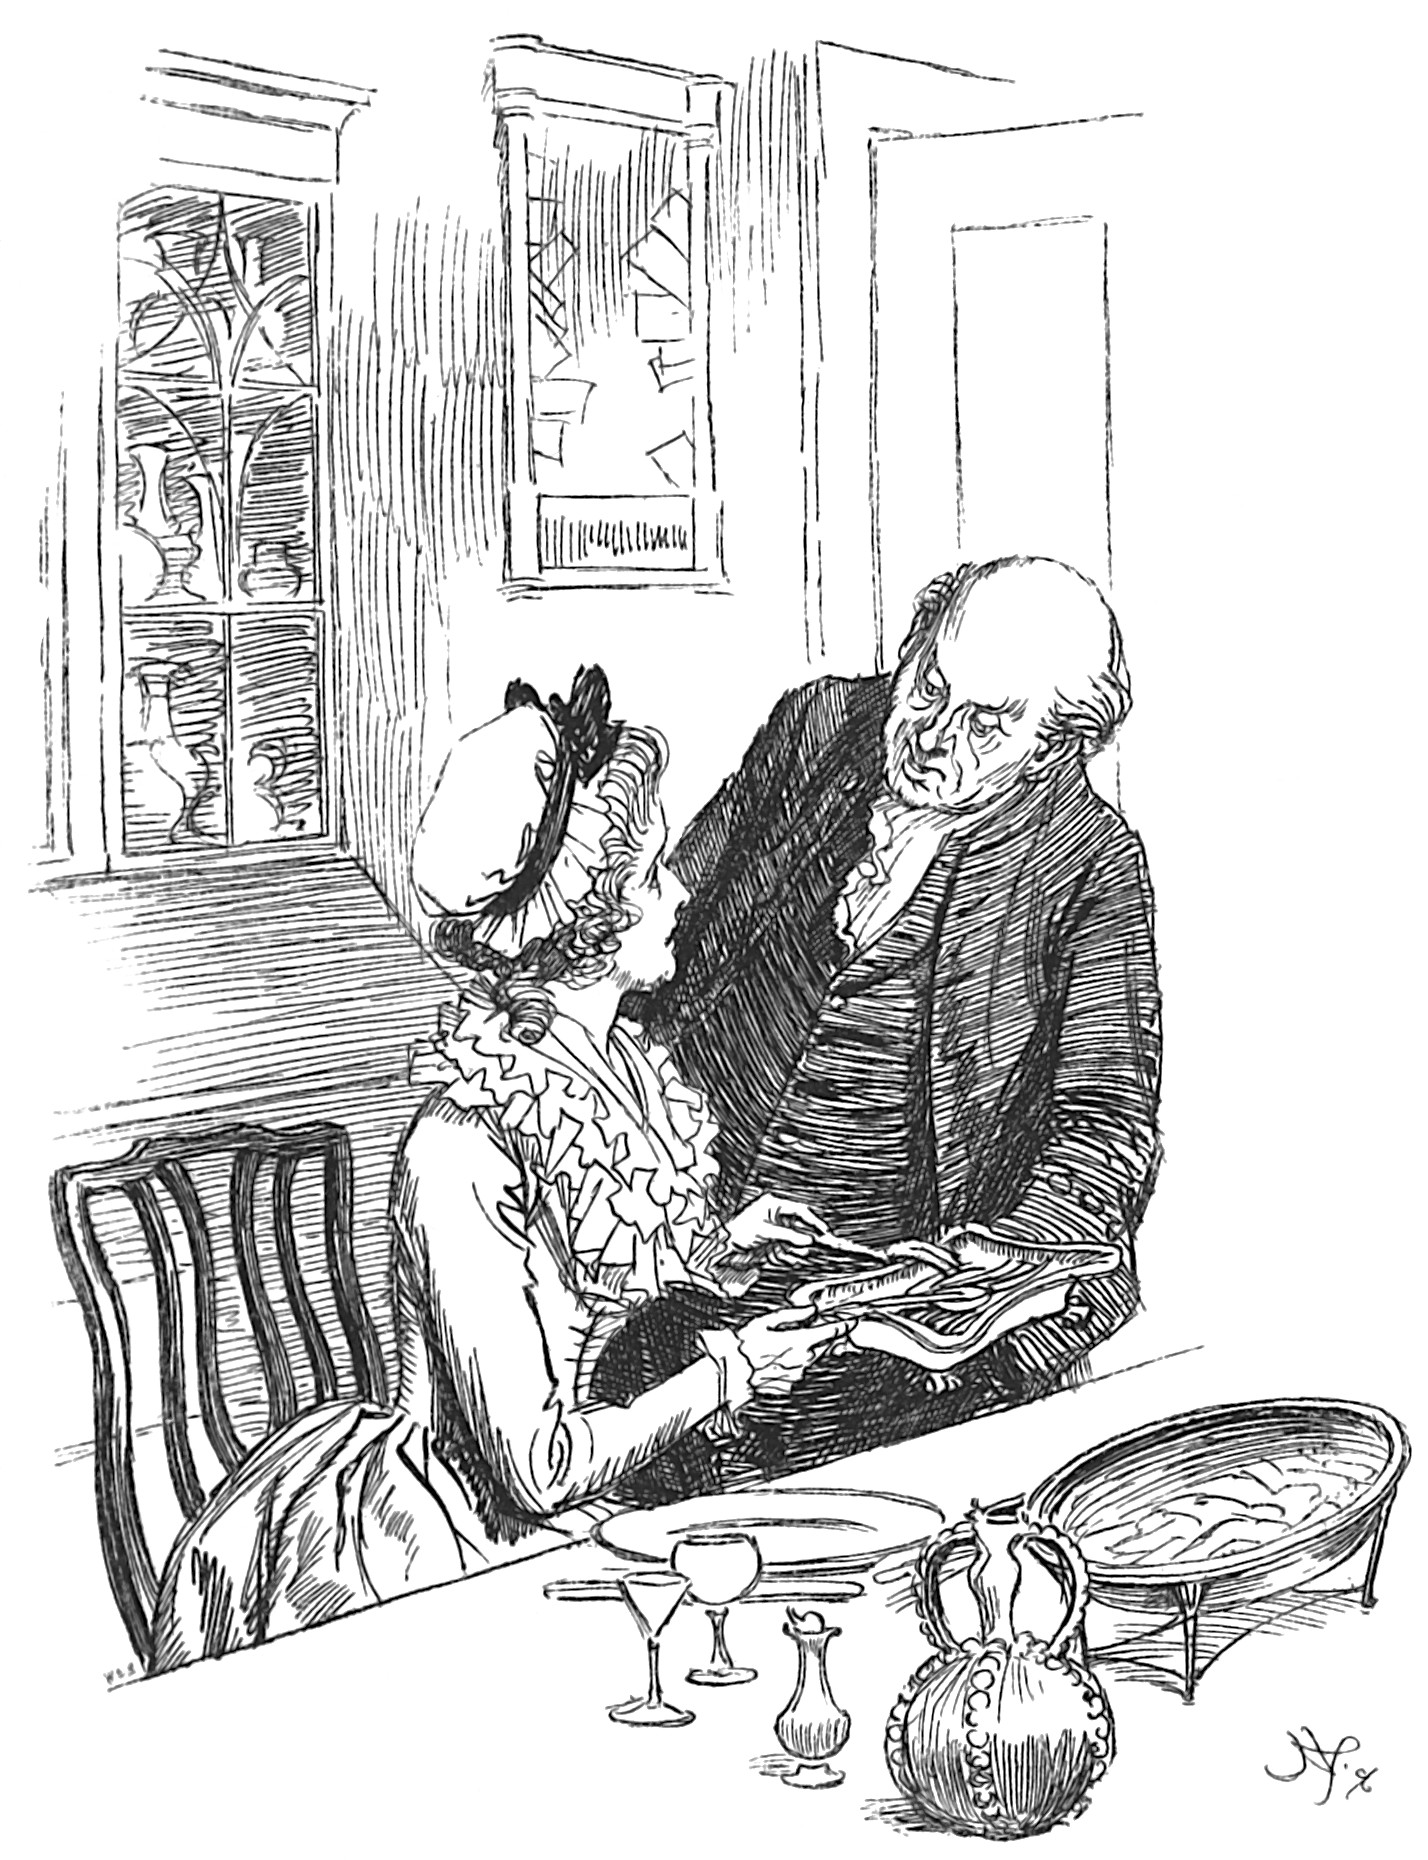
\includegraphics[width=\linewidth]{47married}
\caption{»I suppose you know, ma’am, that Mr Ferrars is married.«}
\end{figure}

Marianne gave a violent start, fixed her eyes upon Elinor, saw her turning pale, and fell back in her chair in hysterics. Mrs Dashwood, whose eyes, as she answered the servant’s inquiry, had intuitively taken the same direction, was shocked to perceive by Elinor’s countenance how much she really suffered, and a moment afterwards, alike distressed by Marianne’s situation, knew not on which child to bestow her principal attention.

The servant, who saw only that Miss Marianne was taken ill, had sense enough to call one of the maids, who, with Mrs Dashwood’s assistance, supported her into the other room. By that time, Marianne was rather better, and her mother leaving her to the care of Margaret and the maid, returned to Elinor, who, though still much disordered, had so far recovered the use of her reason and voice as to be just beginning an inquiry of Thomas, as to the source of his intelligence. Mrs Dashwood immediately took all that trouble on herself; and Elinor had the benefit of the information without the exertion of seeking it.

»Who told you that Mr Ferrars was married, Thomas?«

»I see Mr Ferrars myself, ma’am, this morning in Exeter, and his lady too, Miss Steele as was. They was stopping in a chaise at the door of the New London Inn, as I went there with a message from Sally at the Park to her brother, who is one of the post-boys. I happened to look up as I went by the chaise, and so I see directly it was the youngest Miss Steele; so I took off my hat, and she knew me and called to me, and inquired after you, ma’am, and the young ladies, especially Miss Marianne, and bid me I should give her compliments and Mr Ferrars’s, their best compliments and service, and how sorry they was they had not time to come on and see you, but they was in a great hurry to go forwards, for they was going further down for a little while, but howsever, when they come back, they’d make sure to come and see you.«

»But did she tell you she was married, Thomas?«

»Yes, ma’am. She smiled, and said how she had changed her name since she was in these parts. She was always a very affable and free-spoken young lady, and very civil behaved. So, I made free to wish her joy.«

»Was Mr Ferrars in the carriage with her?«

»Yes, ma’am, I just see him leaning back in it, but he did not look up;—he never was a gentleman much for talking.«

Elinor’s heart could easily account for his not putting himself forward; and Mrs Dashwood probably found the same explanation.

»Was there no one else in the carriage?«

»No, ma’am, only they two.«

»Do you know where they came from?«

»They come straight from town, as Miss Lucy—Mrs Ferrars told me.«

»And are they going farther westward?«

»Yes, ma’am—but not to bide long. They will soon be back again, and then they’d be sure and call here.«

Mrs Dashwood now looked at her daughter; but Elinor knew better than to expect them. She recognised the whole of Lucy in the message, and was very confident that Edward would never come near them. She observed in a low voice, to her mother, that they were probably going down to Mr Pratt’s, near Plymouth.

Thomas’s intelligence seemed over. Elinor looked as if she wished to hear more.

»Did you see them off, before you came away?«

»No, ma’am—the horses were just coming out, but I could not bide any longer; I was afraid of being late.«

»Did Mrs Ferrars look well?«

»Yes, ma’am, she said how she was very well; and to my mind she was always a very handsome young lady—and she seemed vastly contented.«

Mrs Dashwood could think of no other question, and Thomas and the tablecloth, now alike needless, were soon afterwards dismissed. Marianne had already sent to say, that she should eat nothing more. Mrs Dashwood’s and Elinor’s appetites were equally lost, and Margaret might think herself very well off, that with so much uneasiness as both her sisters had lately experienced, so much reason as they had often had to be careless of their meals, she had never been obliged to go without her dinner before.

When the dessert and the wine were arranged, and Mrs Dashwood and Elinor were left by themselves, they remained long together in a similarity of thoughtfulness and silence. Mrs Dashwood feared to hazard any remark, and ventured not to offer consolation. She now found that she had erred in relying on Elinor’s representation of herself; and justly concluded that every thing had been expressly softened at the time, to spare her from an increase of unhappiness, suffering as she then had suffered for Marianne. She found that she had been misled by the careful, the considerate attention of her daughter, to think the attachment, which once she had so well understood, much slighter in reality, than she had been wont to believe, or than it was now proved to be. She feared that under this persuasion she had been unjust, inattentive, nay, almost unkind, to her Elinor;—that Marianne’s affliction, because more acknowledged, more immediately before her, had too much engrossed her tenderness, and led her away to forget that in Elinor she might have a daughter suffering almost as much, certainly with less self-provocation, and greater fortitude.